\documentclass[11pt,aspectratio=169]{beamer}

\usetheme{Madrid}
\usecolortheme{seahorse}

\usepackage[utf8]{inputenc}
\usepackage{amsmath,amssymb}
\usepackage{algpseudocode}
\usepackage{algorithmicx}
\usepackage{xcolor}
\usepackage{listings}
\usepackage{booktabs}
\usepackage{tikz}
\usetikzlibrary{arrows.meta,positioning,fit,backgrounds}

\setbeamertemplate{navigation symbols}{}
\setbeamertemplate{footline}[frame number]

\lstdefinestyle{py}{
  language=Python,
  basicstyle=\ttfamily\scriptsize,
  keywordstyle=\color{blue!70!black}\bfseries,
  commentstyle=\color{gray},
  stringstyle=\color{green!40!black},
  showstringspaces=false,
  breaklines=true,
  numbers=left,
  numberstyle=\tiny\color{gray},
  frame=single,
  xleftmargin=1.5em,
  aboveskip=0.3em,
  belowskip=0.3em
}

\title{LeetCode Deep Dive}
\subtitle{From First Instinct to Optimal Algorithm: Union-Find and Graph DFS in Practice\\
\small Week 3 Supplement -- TOAE209/TOAH209: Design and Analysis of Algorithms}
\author{Foreign Trade University}
\date{}

\begin{document}

% ---------------------------------------------------------------
\begin{frame}
  \titlepage
\end{frame}
% ---------------------------------------------------------------

\begin{frame}{Outline}
  \tableofcontents
\end{frame}

% =================================================================
\section{A Framework for Attacking a New Graph Problem}
% =================================================================

\begin{frame}{Why walk through LeetCode problems?}
  \begin{itemize}
    \item This week's \texttt{LEETCODE.md} list already gives you ten Week 3 problems to
    \emph{practice on your own}. This deck instead \textbf{narrates the thinking process}
    for two of them, end to end, so you can reuse the process on the other eight.
    \item We pick one \textcolor{blue!50!black}{\textbf{Medium}} (\emph{Redundant
    Connection}) and one \textcolor{red!60!black}{\textbf{Hard}} (\emph{Critical
    Connections in a Network}) -- both graph problems, both solved optimally with tools
    from this week's lecture: \textbf{Union-Find} and \textbf{DFS}.
    \item Spoiler: the two problems turn out to be \textbf{mirror images} of each other --
    one finds an edge that \emph{is} on a cycle (safe to delete), the other finds every
    edge that is \emph{not} on any cycle (a bridge -- unsafe to delete).
  \end{itemize}
\end{frame}

\begin{frame}{The four-step process we will repeat twice}
  \begin{enumerate}
    \item \textbf{First instinct.} Write down the algorithm that follows most directly
    from re-reading the problem statement -- usually a simulate-it-literally or
    try-every-possibility approach.
    \item \textbf{Measure why it hurts.} Compute the actual complexity, plug in the
    problem's constraints, and see the number blow up.
    \item \textbf{Find the structural insight.} Ask: \emph{what property of the problem
    lets me avoid redoing that work?} This is almost always a graph-theoretic fact
    (a counting argument, a cycle/tree property, a monotonicity).
    \item \textbf{Implement the optimal algorithm}, trace it by hand on a small example,
    then look for the \emph{programming-level} (not algorithmic) tricks that make the
    implementation itself correct and fast.
  \end{enumerate}
  \begin{alertblock}{This mirrors the course}
    Steps 1--3 are exactly the ``upper bound via a clever algorithm'' story from this
    week's Union-Find lecture ($O(n^2) \to O(n \log n) \to O(n\,\alpha(n))$); step 4 is
    what turns a correct algorithm into working code.
  \end{alertblock}
\end{frame}

% =================================================================
\section{Problem 1 (Medium): Redundant Connection}
% =================================================================

\begin{frame}{Problem statement}
  \begin{block}{LeetCode 684 -- Redundant Connection (\textcolor{blue!50!black}{Medium})}
    A tree with $n$ nodes labeled $1, \dots, n$ has exactly $n-1$ edges. You are given
    the tree's edge list \emph{plus one extra edge}, so the input has exactly $n$ edges
    and contains exactly \textbf{one cycle}. Return an edge that can be removed so the
    graph becomes a tree again. If several edges lie on the cycle, return the one that
    occurs \textbf{last} in the input.
  \end{block}
  \begin{itemize}
    \item Constraints (LeetCode): $3 \le n \le 1000$, exactly $n$ edges, no self-loops,
    no duplicate edges, input represents a connected graph.
    \item This is precisely ``detect the one cycle in an otherwise-tree graph,'' the
    undirected cycle-detection question from this week's lecture.
  \end{itemize}
\end{frame}

\begin{frame}{Worked example}
  \begin{columns}
  \begin{column}{0.46\textwidth}
  \begin{center}
  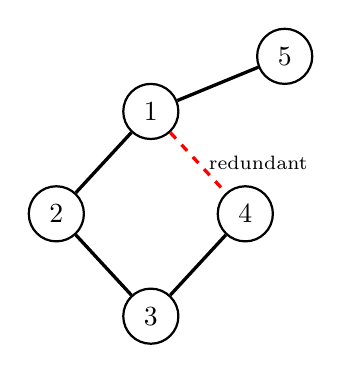
\begin{tikzpicture}[
      vtx/.style={circle, draw, thick, minimum size=7mm},
      >=Stealth]
    \node[vtx] (n1) at (0,1.3)   {1};
    \node[vtx] (n2) at (-1.2,0)  {2};
    \node[vtx] (n3) at (0,-1.3)  {3};
    \node[vtx] (n4) at (1.2,0)   {4};
    \node[vtx] (n5) at (1.7,2.0) {5};
    \draw[very thick] (n1)--(n2);
    \draw[very thick] (n2)--(n3);
    \draw[very thick] (n3)--(n4);
    \draw[very thick, red, dashed] (n1)--(n4)
      node[midway, right, font=\scriptsize, black]{redundant};
    \draw[very thick] (n1)--(n5);
  \end{tikzpicture}
  \end{center}
  \end{column}
  \begin{column}{0.54\textwidth}
  \small
  \texttt{connections = [[1,2],[2,3],[3,4],\allowbreak[1,4],[1,5]]}
  \begin{itemize}
    \item Edges $1$--$2$--$3$--$4$--$1$ form the unique cycle.
    \item Edge $1$--$5$ is a harmless pendant, added \emph{after} the cycle already
    closed.
    \item \textbf{Answer:} $[1,4]$ -- the edge that, when scanned left to right, is the
    one that closes the cycle.
  \end{itemize}
  \end{column}
  \end{columns}
\end{frame}

\begin{frame}{First instinct: try removing each candidate}
  \begin{block}{Most direct reading of the problem}
    ``Return an edge whose removal makes it a tree'' $\Rightarrow$ for each edge $e$
    (scanning from the \emph{end}, since ties break toward the last edge), remove $e$
    and check: is the remaining graph connected with exactly $n-1$ edges?
  \end{block}
  \begin{algorithmic}[1]
    \For{$i \gets m-1$ \textbf{downto} $0$} \Comment{$m = n$ here}
      \State $G' \gets$ all edges except edge $i$
      \If{\Call{IsConnected}{$G'$} via BFS/DFS from node $1$}
        \State \Return edge $i$
      \EndIf
    \EndFor
  \end{algorithmic}
\end{frame}

\begin{frame}{Why this is bad}
  \begin{itemize}
    \item Each connectivity check is a full BFS/DFS: $O(n+m) = O(n)$ (since $m=n$ here).
    \item In the worst case (the cycle is the \emph{whole} graph, e.g.\ a Hamiltonian
    cycle $1\text{-}2\text{-}\cdots\text{-}n\text{-}1$), you must try up to $n$ candidate
    removals before finding the right one.
    \item Total: $O(n) \times O(n) = O(n^2)$ -- and you \textbf{rebuild the entire
    connectivity picture from scratch} on every single trial, throwing away almost all
    of the previous trial's work.
  \end{itemize}
  \begin{alertblock}{The smell to notice}
    Whenever an algorithm says ``try removing/adding $X$, then recheck everything,''
    ask: \emph{does removing $X$ actually change much, or am I recomputing the same
    answer $n$ times?} That question is what leads to the insight below.
  \end{alertblock}
\end{frame}

\begin{frame}{The structural insight}
  \begin{itemize}
    \item The input has \emph{exactly} $n$ edges on $n$ nodes and is connected
    $\Rightarrow$ it is a tree ($n-1$ edges) plus \textbf{exactly one} extra edge
    $\Rightarrow$ \textbf{exactly one cycle exists, and exactly one edge in the whole
    scan will ever connect two nodes that are already in the same component.}
    \item So you never need to \emph{remove and recheck} anything. Just \textbf{add
    edges left to right} and watch for the first moment two endpoints are already
    connected -- that edge is provably the (unique) answer.
    \item This is exactly the graph-traversal insight from this week's lecture:
    ``a new edge closes a cycle iff its endpoints are already in the same connected
    component.'' Union-Find answers \emph{that specific question} in near-constant time.
  \end{itemize}
\end{frame}

\begin{frame}{Optimal algorithm: single Union-Find pass}
  \footnotesize
  \begin{algorithmic}[1]
    \Function{Find}{$x$}
      \While{$parent[x] \neq x$}
        \State $parent[x] \gets parent[parent[x]]$ \Comment{path halving}
        \State $x \gets parent[x]$
      \EndWhile
      \State \Return $x$
    \EndFunction
    \Function{RedundantConnection}{edges}
      \State initialize $parent[i] \gets i$ for all nodes
      \For{$(u,v)$ in edges} \Comment{scan left to right}
        \State $r_u, r_v \gets \Call{Find}{u}, \Call{Find}{v}$
        \If{$r_u = r_v$}
          \State \Return $(u,v)$ \Comment{first edge closing the (unique) cycle}
        \EndIf
        \State $parent[r_v] \gets r_u$ \Comment{union}
      \EndFor
    \EndFunction
  \end{algorithmic}
  Cost: $O(n\,\alpha(n))$ with union by rank + path compression -- this week's bound.
\end{frame}

\begin{frame}{Trace on the worked example}
  \small
  \texttt{connections = [[1,2],[2,3],[3,4],[1,4],[1,5]]}
  \begin{center}
  \begin{tabular}{@{}cccccl@{}}
    \toprule
    edge & find(u) & find(v) & same root? & action & components after \\
    \midrule
    $(1,2)$ & $1$ & $2$ & no  & union & $\{1,2\}, \{3\}, \{4\}, \{5\}$ \\
    $(2,3)$ & $1$ & $3$ & no  & union & $\{1,2,3\}, \{4\}, \{5\}$ \\
    $(3,4)$ & $1$ & $4$ & no  & union & $\{1,2,3,4\}, \{5\}$ \\
    $(1,4)$ & $1$ & $1$ & \textbf{yes} & \textbf{stop} & -- \\
    \bottomrule
  \end{tabular}
  \end{center}
  \begin{exampleblock}{Answer}
    Edge $(1,4)$ is the first (and, by the problem's guarantee, only) edge whose
    endpoints already share a root. Edge $(1,5)$ is never even reached.
  \end{exampleblock}
\end{frame}

\begin{frame}{Complexity: naive vs.\ optimal}
  \begin{center}
  \begin{tabular}{@{}lll@{}}
    \toprule
    Approach & Time & Idea \\
    \midrule
    Remove-and-recheck (naive) & $O(n^2)$ & re-run BFS/DFS after each trial removal \\
    Rebuild via BFS/DFS components & $O(n^2)$ & re-run BFS/DFS after each new edge \\
    \textbf{Union-Find, single pass} & $\boldsymbol{O(n\,\alpha(n))}$ & incremental,
    online connectivity test \\
    \bottomrule
  \end{tabular}
  \end{center}
  \begin{itemize}
    \item Note that plain BFS/DFS recomputation \emph{per edge} is also $O(n^2)$: it is
    the \emph{online} nature of the query (``are $u,v$ connected \emph{right now}, after
    only some edges have been added?'') that Union-Find is built for -- not just raw
    graph size.
  \end{itemize}
\end{frame}

\begin{frame}[fragile]{Python implementation (part 1: the Union-Find class)}
  \begin{lstlisting}[style=py]
class UnionFind:
    def __init__(self, n):
        self.parent = list(range(n + 1))   # 1-indexed nodes
        self.rank = [0] * (n + 1)

    def find(self, x):
        while self.parent[x] != x:
            self.parent[x] = self.parent[self.parent[x]]  # path halving
            x = self.parent[x]
        return x

    def union(self, a, b):
        ra, rb = self.find(a), self.find(b)
        if ra == rb:
            return False              # already connected: cycle-closing edge
        if self.rank[ra] < self.rank[rb]:
            ra, rb = rb, ra
        self.parent[rb] = ra
        if self.rank[ra] == self.rank[rb]:
            self.rank[ra] += 1
        return True
  \end{lstlisting}
\end{frame}

\begin{frame}[fragile]{Python implementation (part 2: the driver)}
  \begin{lstlisting}[style=py]
def findRedundantConnection(edges):
    uf = UnionFind(len(edges))
    for u, v in edges:
        if not uf.union(u, v):
            return [u, v]
    return []                          # unreachable given the problem's guarantee
  \end{lstlisting}
  \vspace{0.5em}
  The very first edge that fails to \texttt{union} (because its endpoints are already
  joined) is returned immediately -- no need to look at the rest of the list.
\end{frame}

\begin{frame}{Implementation tips \& tricks (the programming side)}
  \small
  These are \emph{not} about the algorithm's Big-O -- the algorithm above is already
  optimal. They are about turning it into code that is actually correct and fast.
  \begin{itemize}
    \item \textbf{Iterative \texttt{find}, not recursive.} A recursive \texttt{find}
    walks up the parent chain via function calls. On an adversarial input where edges
    are added as a long chain ($1\text{-}2, 2\text{-}3, \dots$) \emph{without} union by
    rank, the recursion depth equals the chain length -- for $n$ near Python's default
    recursion limit ($1000$), that is a real \texttt{RecursionError}, not just a
    slowdown. The \texttt{while} loop above has no such limit.
    \item \textbf{Path halving vs.\ full path compression.} \texttt{parent[x] =
    parent[parent[x]]} inside the loop is a cheap one-line trick that still gives the
    same $O(\alpha(n))$ amortized bound as full recursive compression, with no extra
    pass over the path.
    \item \textbf{Union by rank matters even for small $n$.} Without it, a chain input
    produces a chain-shaped tree ($O(n)$ per \texttt{find}); with it, tree height is
    provably $O(\log n)$ even before compression kicks in.
  \end{itemize}
\end{frame}

% =================================================================
\section{Problem 2 (Hard): Critical Connections in a Network}
% =================================================================

\begin{frame}{Problem statement}
  \begin{block}{LeetCode 1192 -- Critical Connections in a Network (\textcolor{red!60!black}{Hard})}
    There are $n$ servers labeled $0,\dots,n-1$ connected by an undirected, connected
    graph with edge list \texttt{connections} (no self-loops, no duplicate edges).
    A \textbf{critical connection} (a \textbf{bridge}) is an edge whose removal
    disconnects the network. Return \emph{all} critical connections.
  \end{block}
  \begin{itemize}
    \item Constraints (LeetCode): $n \le 10^5$, up to $10^5$ edges.
    \item This is the exact mirror of Problem 1: instead of finding the one edge that
    \emph{is} on a cycle, find every edge that is \textbf{on no cycle at all}.
  \end{itemize}
\end{frame}

\begin{frame}{Worked example}
  \begin{columns}
  \begin{column}{0.46\textwidth}
  \begin{center}
  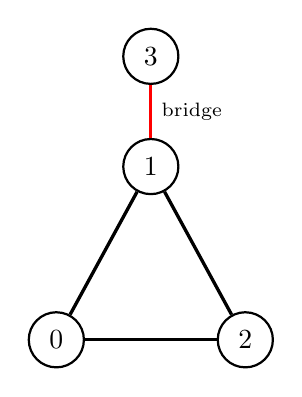
\begin{tikzpicture}[
      vtx/.style={circle, draw, thick, minimum size=7mm},
      >=Stealth]
    \node[vtx] (n0) at (-1.2,-1) {0};
    \node[vtx] (n1) at (0,1.2)   {1};
    \node[vtx] (n2) at (1.2,-1)  {2};
    \node[vtx] (n3) at (0,2.6)  {3};
    \draw[very thick] (n0)--(n1);
    \draw[very thick] (n1)--(n2);
    \draw[very thick] (n2)--(n0);
    \draw[very thick, red] (n1)--(n3)
      node[midway, right, font=\scriptsize, black]{bridge};
  \end{tikzpicture}
  \end{center}
  \end{column}
  \begin{column}{0.54\textwidth}
  \small
  \texttt{connections = [[0,1],[1,2],\allowbreak[2,0],[1,3]]}
  \begin{itemize}
    \item $0,1,2$ form a triangle: every edge among them lies on a cycle, so removing
    any \emph{one} of them still leaves the network connected.
    \item Edge $1$--$3$ is a pendant, on \textbf{no} cycle: removing it strands server
    $3$.
    \item \textbf{Answer:} $[[1,3]]$.
  \end{itemize}
  \end{column}
  \end{columns}
\end{frame}

\begin{frame}{First instinct: remove each edge and recheck}
  \begin{block}{Most direct reading of the problem}
    ``An edge is critical if removing it disconnects the graph'' $\Rightarrow$ for each
    edge, remove it, run BFS/DFS to see if the graph is still connected, then put the
    edge back.
  \end{block}
  \begin{algorithmic}[1]
    \For{each edge $e \in$ connections}
      \State $G' \gets G$ with $e$ removed
      \If{\textbf{not} \Call{IsConnected}{$G'$}}
        \State add $e$ to the answer
      \EndIf
    \EndFor
  \end{algorithmic}
\end{frame}

\begin{frame}{Why this is bad}
  \begin{itemize}
    \item Each connectivity check costs $O(n+m)$.
    \item There are $m$ edges to try $\Rightarrow O(m(n+m))$ total.
    \item Plug in the actual constraints: $n = m = 10^5 \Rightarrow$ roughly
    $10^5 \times 2 \times 10^5 = 2\times10^{10}$ operations. Even at $10^9$ simple
    operations/second this is $\sim 20$ seconds of raw work -- and Python is far slower
    than that per operation. This \textbf{will} time out.
  \end{itemize}
  \begin{alertblock}{The smell to notice (again)}
    Same pattern as Problem 1: ``remove one thing, recheck everything from scratch,
    repeat for every thing.'' That is always a hint that most of the recomputation is
    unnecessary -- the question is \emph{what invariant} lets you reuse work.
  \end{alertblock}
\end{frame}

\begin{frame}{Structural insight \#1: only tree edges can be bridges}
  \begin{itemize}
    \item Run one DFS from any start node; every edge is either a \textbf{tree edge}
    (first time you reach that node) or a \textbf{back edge} (an edge to an already-visited
    ancestor -- this week's cycle-detection idea, extended to undirected graphs).
    \item A back edge, by definition, sits on a cycle (the tree path down plus the back
    edge itself) $\Rightarrow$ removing it \textbf{cannot} disconnect the graph. Back
    edges are \emph{never} bridges.
    \item This alone prunes the $m$ candidates down to at most $n-1$ tree edges -- but we
    still need an $O(1)$-ish test \emph{per tree edge}, not another full BFS/DFS each
    time.
  \end{itemize}
\end{frame}

\begin{frame}{Structural insight \#2: discovery time and low-link}
  For each node $u$, computed during one single DFS:
  \begin{itemize}
    \item $tin[u]$: the time (a counter, incremented once per visit) when $u$ is first
    discovered.
    \item $low[u]$: the \textbf{smallest} $tin$ value reachable from $u$'s subtree using
    at most \emph{one} back edge -- i.e., how far back up the tree can this subtree
    ``reach'' without using the edge to its parent.
    \[
      low[u] = \min\Big(tin[u],\ \min_{(u,v)\text{ back edge}} tin[v],\ \min_{(u,c)\text{
      tree edge}} low[c]\Big)
    \]
    \item \textbf{Bridge test:} tree edge $(parent, child)$ is a bridge
    $\iff low[child] > tin[parent]$ -- i.e., $child$'s entire subtree has \textbf{no}
    back edge escaping past $parent$.
  \end{itemize}
\end{frame}

\begin{frame}{DFS trace on the worked example}
  \scriptsize
  Adjacency: $0\!:\!\{1,2\}$, $1\!:\!\{0,2,3\}$, $2\!:\!\{1,0\}$, $3\!:\!\{1\}$. DFS from
  node $0$, timer starts at $0$.
  \begin{center}
  \begin{tabular}{@{}c p{3.1cm} c c p{3.6cm}@{}}
    \toprule
    step & event & $tin$ & $low$ & remark \\
    \midrule
    1 & discover $0$ & $0$ & $0$ & start \\
    2 & discover $1$ (tree $0{-}1$) & $1$ & $1$ & \\
    3 & discover $2$ (tree $1{-}2$) & $2$ & $2$ & \\
    4 & edge $2{-}0$: $0$ already visited, not parent & -- & $low[2]{=}0$ & back edge:
    $low[2]\gets\min(2,tin[0]{=}0)$ \\
    5 & return $2\to1$ & -- & $low[1]{=}0$ & $low[2]{=}0 \not> tin[1]{=}1$: not a bridge \\
    6 & discover $3$ (tree $1{-}3$) & $3$ & $3$ & \\
    7 & return $3\to1$ & -- & $low[1]{=}0$ & $low[3]{=}3 > tin[1]{=}1$: \textbf{bridge!} \\
    8 & return $1\to0$ & -- & $low[0]{=}0$ & $low[1]{=}0 \not> tin[0]{=}0$: not a bridge \\
    \bottomrule
  \end{tabular}
  \end{center}
  Result: only $(1,3)$ satisfies $low[child] > tin[parent]$ -- matches the expected
  output $[[1,3]]$.
\end{frame}

\begin{frame}{Optimal algorithm: pseudocode}
  \footnotesize
  Run \Call{DFS}{$s$, $-1$} from any unvisited $s$ (repeat for every unvisited vertex,
  in case the graph is disconnected):
  \begin{algorithmic}[1]
    \Function{DFS}{$u$, parentEdge}
      \State $tin[u] \gets low[u] \gets timer$;\ $timer \gets timer+1$; mark $u$ visited
      \For{each edge $(u,v)$ with id $e$ incident to $u$}
        \If{$e = parentEdge$} \textbf{continue} \Comment{never re-cross the entry edge}
        \ElsIf{$v$ unvisited}
          \State \Call{DFS}{$v$, $e$}
          \State $low[u] \gets \min(low[u], low[v])$
          \If{$low[v] > tin[u]$} report $(u,v)$ as a bridge \EndIf
        \Else
          \State $low[u] \gets \min(low[u], tin[v])$ \Comment{back edge: relax}
        \EndIf
      \EndFor
    \EndFunction
  \end{algorithmic}
  $O(n+m)$ total -- the same traversal bound as plain BFS/DFS this week, plus two
  $O(1)$ bookkeeping arrays.
\end{frame}

\begin{frame}{Complexity: naive vs.\ optimal}
  \begin{center}
  \begin{tabular}{@{}lll@{}}
    \toprule
    Approach & Time & At $n=m=10^5$ \\
    \midrule
    Remove edge + recheck connectivity & $O(m(n+m))$ & $\sim 2\times 10^{10}$ ops \\
    Prune to tree edges, still recheck each & $O(n(n+m))$ & $\sim 2\times 10^{10}$ ops \\
    \textbf{Single DFS with $tin$/$low$} & $\boldsymbol{O(n+m)}$ & $\sim 2\times 10^5$
    ops \\
    \bottomrule
  \end{tabular}
  \end{center}
  Five orders of magnitude apart -- the difference between ``times out'' and
  ``instant,'' purely from finding the right invariant ($low[child] > tin[parent]$)
  instead of brute-force rechecking.
\end{frame}

\begin{frame}[fragile]{Python implementation (part 1: building the graph)}
  \begin{lstlisting}[style=py]
def criticalConnections(n, connections):
    graph = [[] for _ in range(n)]
    for edge_id, (u, v) in enumerate(connections):
        graph[u].append((v, edge_id))
        graph[v].append((u, edge_id))     # store the edge's own id, not just "parent"

    tin = [-1] * n
    low = [0] * n
    timer = 0
    bridges = []
  \end{lstlisting}
  Storing the \textbf{edge id} alongside each neighbor (not just the neighbor itself)
  is what lets us correctly skip ``the edge we just came from'' in the next slide.
\end{frame}

\begin{frame}[fragile]{Python implementation (part 2a: descend / relax)}
  \begin{lstlisting}[style=py,aboveskip=0pt,belowskip=0pt]
    for root in range(n):
        if tin[root] != -1:
            continue
        stack = [[root, -1, 0]]       # [node, incoming_edge_id, neighbor_cursor]
        tin[root] = low[root] = timer
        timer += 1
        while stack:
            node, in_edge, idx = stack[-1]
            if idx < len(graph[node]):
                stack[-1][2] += 1                # advance cursor before using it
                nxt, eid = graph[node][idx]
                if eid == in_edge:
                    continue                      # don't re-cross the entry edge
                if tin[nxt] == -1:                # tree edge: descend
                    tin[nxt] = low[nxt] = timer
                    timer += 1
                    stack.append([nxt, eid, 0])
                else:                              # back edge: relax
                    low[node] = min(low[node], tin[nxt])
  \end{lstlisting}
\end{frame}

\begin{frame}[fragile]{Python implementation (part 2b: return / record bridges)}
  \begin{lstlisting}[style=py]
            else:
                stack.pop()                            # subtree of node fully explored
                if stack:
                    parent = stack[-1][0]
                    low[parent] = min(low[parent], low[node])
                    if low[node] > tin[parent]:
                        bridges.append(connections[in_edge])
    return bridges
  \end{lstlisting}
  \vspace{0.5em}
  This \texttt{else} branch fires once a node's neighbor cursor reaches the end of its
  list -- the iterative equivalent of a recursive call \emph{returning}: relax the
  parent's \texttt{low} and apply the bridge test right there.
\end{frame}

\begin{frame}{Implementation tips \& tricks (the programming side)}
  \small
  \begin{itemize}
    \item \textbf{Recursive DFS will crash on this problem, not just run slowly.} A
    textbook-clean recursive version of the pseudocode above hits Python's default
    recursion limit ($\approx 1000$) whenever the graph contains a path of $> 1000$
    nodes -- entirely possible at $n = 10^5$. Raising
    \texttt{sys.setrecursionlimit} alone can still segfault (the \emph{C} stack, not
    just Python's counter, overflows); the robust fix is either running the recursive
    version on a thread with a manually enlarged \texttt{threading.stack\_size()}, or --
    as above -- converting the recursion into an \textbf{explicit stack} that stores a
    resumable cursor into each node's neighbor list.
    \item \textbf{Track the incoming edge's id, not the parent node.} If a graph ever
    has multiple edges between the same pair (not this problem, but common in the
    ``directed'' sequel \emph{Redundant Connection II}), ``skip any edge back to the
    parent'' silently discards a legitimate second edge. Skipping by exact \texttt{edge\_id}
    is correct in general; skipping by parent \emph{node} only happens to be correct
    here because the input has no duplicate edges.
  \end{itemize}
\end{frame}

\begin{frame}{Implementation tips \& tricks (continued)}
  \small
  \begin{itemize}
    \item \textbf{Preallocate arrays, don't grow dictionaries.} \texttt{tin = [-1] * n}
    and \texttt{low = [0] * n} are $O(1)$-indexed from the start; a \texttt{dict} that
    grows one key at a time carries hashing overhead that is measurable at $n=10^5$ in
    Python.
    \item \textbf{\texttt{graph = [[] for \_ in range(n)]}, not \texttt{defaultdict(list)}.}
    Both work, but a plain list avoids \texttt{defaultdict}'s per-access dispatch inside
    the hottest loop in the program (every edge is touched twice, once per endpoint).
    \item \textbf{A one-element mutable ``cursor'' per stack frame is what makes the
    stack resumable.} The trick that makes the iterative version behave exactly like
    recursion-with-a-return-address is storing \emph{where you left off} (\texttt{idx})
    in each frame, so popping back up resumes the parent's loop instead of restarting it.
  \end{itemize}
\end{frame}

% =================================================================
\section{Summary}
% =================================================================

\begin{frame}{Summary: two problems, one lesson}
  \footnotesize
  \begin{enumerate}
    \item \textbf{Redundant Connection} finds the one edge that \emph{is} on the graph's
    (unique) cycle -- solved by Union-Find, because the question is ``are these two
    nodes already connected \emph{right now}?'', asked incrementally as edges arrive.
    \item \textbf{Critical Connections} finds every edge that is \emph{on no cycle at
    all} -- solved by a single DFS with $tin$/$low$, because the question is a
    \emph{static} property of the whole graph, best answered by one traversal that
    remembers what it has already seen.
    \item Both times, the naive instinct was ``recompute connectivity from scratch for
    every candidate''; both times, the fix was the same shape: \textbf{find the
    invariant that makes one pass enough} -- exactly the move this week's lecture made
    going from ``recheck the whole tree'' to $O(m\,\alpha(n))$ Union-Find.
    \item The implementation tricks (iterative \texttt{find}/DFS, edge-id tracking,
    preallocated arrays) are a second, independent layer: even the \emph{optimal
    algorithm} can fail in practice if the code hits language-level limits like
    recursion depth.
  \end{enumerate}
  \begin{alertblock}{Keep practicing}
    \texttt{LEETCODE.md} lists eight more Week 3 problems (\emph{Number of Islands},
    \emph{Course Schedule}, \emph{Graph Valid Tree}, \emph{Accounts Merge}, \dots) --
    try applying the same four-step process to each of them.
  \end{alertblock}
\end{frame}

\end{document}
